\documentclass[../defence.tex]{subfiles}
\begin{document}

  \begin{frame}{Ganzzahliger Quanten Hall Effekt (QHE) in bischichtigem Graphen II}
    \begin{columns}[onlytextwidth, T]
      \column{\dimexpr\linewidth / 6 * 3}
        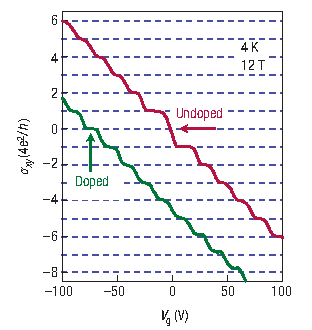
\includegraphics[width=\linewidth]{images/bilayer_qhe.pdf}
      \column{\dimexpr\linewidth / 6 * 3}
        \cite{geim2007}
        \begin{block}{Electrischer Feld Effekt}
          \begin{itemize}
            \item Durch \textit{dopen} wird der Dirac-Punkt verschoben
            \item Entartung wird aufgehoben und die Doppelstufe verschwindet
          \end{itemize}
        \end{block}
    \end{columns}
    \note{
      \begin{itemize}
        \item Stufen für bischichtiges Graphen
        \item Doppelstufe wegen Entartung von $n=0,1$
        \item Durch \textit{Dopen} wird Dirac-Punkt verschoben und Entartung verschwindet $\rightarrow$ elektrische Feld-Effekt
      \end{itemize}
    }
  \end{frame}

\end{document}
